% agent-mafia paper, v2 structure (benchmark-first).
\documentclass[11pt]{article}

\usepackage[T1]{fontenc}
\usepackage[margin=1in]{geometry}
\usepackage{microtype}
\usepackage{booktabs}
\usepackage{tabularx}
\usepackage{array}
\usepackage{amsmath}
\usepackage{graphicx}
\usepackage{float}
\usepackage{placeins}
\usepackage{needspace}
\usepackage{caption}
\usepackage{enumitem}
\usepackage{tikz}
\usetikzlibrary{arrows.meta,positioning,shapes.misc}
\usepackage{pgfplots}
\pgfplotsset{compat=1.18}
\usepackage[round,authoryear]{natbib}
\usepackage{xurl}
\usepackage[colorlinks=true,allcolors=blue!60!black]{hyperref}

\newcommand{\sys}{\textsc{agent-mafia}}
\newcommand{\code}[1]{\texttt{#1}}
\newcolumntype{Y}{>{\raggedright\arraybackslash}X}
\newcolumntype{P}[1]{>{\raggedright\arraybackslash}p{#1}}
\setlength{\parskip}{0pt}
\setlength{\textfloatsep}{12pt plus 2pt minus 2pt}
\setlength{\floatsep}{10pt plus 2pt minus 2pt}
\setlength{\intextsep}{10pt plus 2pt minus 2pt}
\captionsetup[table]{skip=5pt}

\title{Agent-Mafia: An Event-Sourced Environment for Auditing Strategic Claims in Social-Deduction Agents}
\author{Ryan Junejo\\CrashLabs\\\href{mailto:ryan@crashlabs.ai}{ryan@crashlabs.ai}}
\date{September 2026}

\hypersetup{
  pdftitle={Agent-Mafia: An Event-Sourced Environment for Auditing Strategic Claims in Social-Deduction Agents},
  pdfauthor={Ryan Junejo},
  pdfsubject={A verifiable social-deduction environment for language-model agents},
  pdfkeywords={language-model agents, social deduction, Mafia, evaluation environment, event sourcing, claim auditing}
}

\begin{document}
\maketitle

\begin{abstract}
\noindent
Win rate is a weak instrument for social-deduction agents. It scores whole tables when the object of interest is a seat, and it says nothing about whether an agent's statements were true. We present \sys, a deterministic, event-sourced Mafia environment in which agents' role, self-alignment, investigation, and protection claims are extracted from public messages with model assistance and scored deterministically against logged game state. Every game produces a hash-chained, replayable log. In an exploratory study, 12 contemporary language models played 40 eleven-seat games (4,267 agent wakes, 62.55 million tokens). The environment completed every game. First-attempt action validity was 79.45\% overall and ranged from 50.7\% to 100\% by model. In the primary 38-game analysis set, Town ballots targeted a Mafia seat in 60.08\% of valid non-abstentions, against uniform-choice baselines of 28.96\% and 33.53\%; every model's observed point estimate exceeded both. As exploratory, author-adjudicated evidence, 667 quoted claim occurrences map to 433--460 distinct claims, of which 118--120 were verifiably false; 104 of the 120 at the upper end of this linkage range came from Mafia seats, and all 16 from Town seats were power roles claiming to be villagers. An audit of our original claim-verification pipeline found 20 invalid labels among 171, all at the utterance-to-state boundary and none visible to integrity checks. The revised pipeline, audit, logs, and analysis bundle accompany the paper.

\vspace{6pt}\noindent\textit{Keywords}: language-model agents; social deduction; Mafia; evaluation environment; ground-truth verification; event sourcing; claim auditing
\end{abstract}

\section{Introduction}
\label{sec:intro}

Whether an agent wins a game is the natural score for game environments, and for social deduction it is a poor one. A Mafia outcome is shared by eleven seats, so one seat's contribution is confounded by its teammates and its opponents. A Mafia seat can win a game without saying a word and lose one after playing well. And the behaviors that make the game interesting as an evaluation setting, whether the agent acted validly at each turn, whether it voted for the right people under partial information, and whether the things it said about hidden state were true, leave no trace in the scoreline. The analogous move in other game benchmarks is to score how the game was played. Here the object of measurement is what agents said and did, checked against a record the environment keeps of what happened.

On Day~2 of game \code{sweep1-0}, the seat holding the detective role, Bryan, truthfully reported that Night~2's investigation had found Cyan to be Mafia.\footnote{Public log artifacts carry the filename prefix \code{sweep1-}; the paper refers to this data collection as the exploratory campaign.} Cyan, a Mafia seat, replied ``I am the real Detective,'' followed by ``N1: Investigated Trae --- Innocent (Not Mafia)'' and ``N2: Investigated Bryan --- MAFIA,'' and restated both results in a later message. The table executed Bryan by seven votes to two. Town went on to win the game two days later. A win-rate benchmark records a Town win. The event log records a false role claim, two investigation reports with no matching logged action, and a ballot that removed the only truthful detective. Figure~\ref{fig:flow} follows one of those statements from message to verdict.

\begin{figure}[t]
\centering
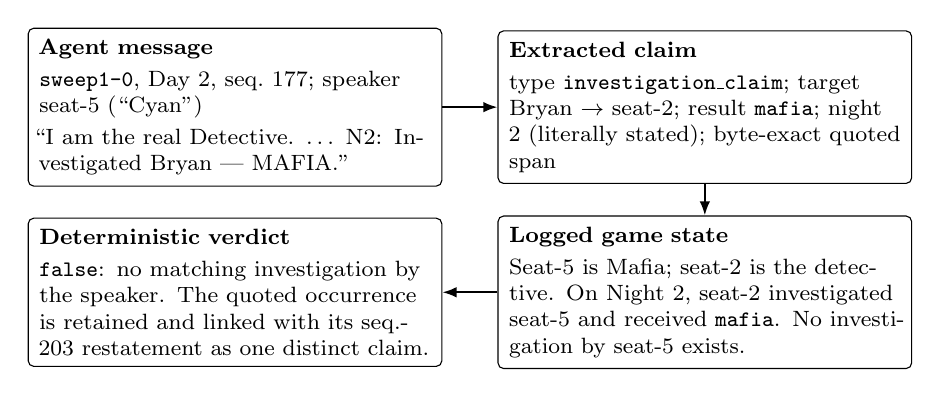
\begin{tikzpicture}[node distance=4mm and 7mm, box/.style={draw, rounded corners=2pt, align=left, font=\footnotesize, inner sep=4pt, text width=0.41\linewidth}, arr/.style={-{Latex[length=1.8mm]}, thick}]
\node[box] (m) {\textbf{Agent message}\\[2pt]\code{sweep1-0}, Day~2, seq.~177; speaker seat-5 (``Cyan'')\\[2pt]``I am the real Detective. \ldots\ N2: Investigated Bryan --- MAFIA.''};
\node[box, right=of m] (p) {\textbf{Extracted claim}\\[2pt]type \code{investigation\_claim}; target Bryan $\to$ seat-2; result \code{mafia}; night 2 (literally stated); byte-exact quoted span};
\node[box, below=of p] (s) {\textbf{Logged game state}\\[2pt]Seat-5 is Mafia; seat-2 is the detective. On Night~2, seat-2 investigated seat-5 and received \code{mafia}. No investigation by seat-5 exists.};
\node[box, left=of s] (v) {\textbf{Deterministic verdict}\\[2pt]\code{false}: no matching investigation by the speaker. The quoted occurrence is retained and linked with its seq.-203 restatement as one distinct claim.};
\draw[arr] (m) -- (p); \draw[arr] (p) -- (s); \draw[arr] (s) -- (v);
\end{tikzpicture}
\caption{One statement through the instrument. Candidate extraction and review are model-assisted; a targeted subset receives author adjudication. Comparison with logged state is deterministic code. The same message yields a false role claim and a second false investigation report, and its later restatement adds claim occurrences without adding distinct claims.}
\label{fig:flow}
\end{figure}

The paper asks three questions. \textbf{RQ1.} Can an event-sourced social-deduction environment make selected strategic claims by language-model agents deterministically checkable, and what does that cost? \textbf{RQ2.} How do contemporary language-model agents behave in such an environment: do they act validly over a long interaction, do their ballots find Mafia seats under partial information, and what captured false claims appear by faction? \textbf{RQ3.} How reliable is the utterance-to-state mapping itself, and what does auditing it reveal?

The contributions are, first, a deterministic Mafia engine with tamper-evident replayable logs, a visibility-filtered event export, and a sampled role-field redaction test on the observation function (\S\ref{sec:env}); second, a claim pipeline whose intermediate semantic record is a first-class artifact, with explicit correction objects, a hash-bound adjudication chain, archived superseded evaluator versions, and a mapping from quoted claim occurrences to distinct claims (\S\ref{sec:env}, \S\ref{sec:setup}); third, the exploratory study and its results (\S\ref{sec:results}); and fourth, a public failure analysis of the pipeline (\S\ref{sec:analysis}). Engine-derived quantities are the quantitative core; captured-claim quantities are exploratory. No model ranking is claimed, and falsity is never treated as evidence of intent.

\section{Related Work}
\label{sec:related}

Social-deduction games entered language-model evaluation as settings where dialogue carries strategy \citep{xu2023werewolf,ogara2023hoodwinked,olson2026liecraft}. These designs differ in what they score. Outcome-scored designs compare win rates or survival \citep{bailis2024werewolf,costa2025minimafia}. Behavior-scored designs label transcript segments, by a judge model or by annotators, for properties such as persuasion or detection \citep{golechha2025amongus,agarwal2025wolf,bauer2026parliamentbench,kao2026hidden}. Statement-grounded designs compare what an agent said with something the environment recorded \citep{karpov2026mafiascope,kang2025miva}. \sys{} is of the third kind.

The closest work is QUACK \citep{yuan2026quack}, which evaluates a multimodal social-deduction agent at the levels of game outcome, behavioral trajectory, and utterance consistency. Its verification pipeline has a language model extract structured, individually checkable claims, caches the extraction, verifies each claim deterministically against environment state, stores the verdict with its supporting evidence, and reports human validation of the extraction step. \sys{} shares that architecture and applies it to a different claim space. QUACK verifies spatial and accusation claims in a multimodal setting; \sys{} verifies the role, self-alignment, investigation, and protection assertions of Mafia. To that shared architecture this paper adds four things: explicit correction objects that carry the human's corrected fields and their provenance into the scorer; hashes that bind every adjudication stage to the exact inputs it ruled on; an archived, superseded pipeline version whose row-level audit will be published beside the corrected one; and a mapping from quoted claim occurrences to distinct claims so that repetition does not inflate totals. \S\ref{sec:analysis} reports what those additions changed in the record.

The vocabulary follows the honesty and deception literature. MASK separates honesty from accuracy by measuring whether a model contradicts what it appears to believe under pressure \citep{ren2025mask}. \citet{park2024aideception} define deception as the systematic inducement of false beliefs in the pursuit of some outcome other than the truth, which requires a target belief and a purpose \citep[see also][]{hagendorff2024deception,shi2026taxonomy}. A logged conflict between an utterance and the game state supplies falsity and nothing more. The paper therefore counts verifiably false distinct claims, keeps them role-conditioned, and reserves deception for case discussion.

\section{The Agent-Mafia Environment}
\label{sec:env}

\subsection{Task and rules}

A game seats eleven agents: three Mafia, one doctor, one detective, and six villagers. Roles and synthetic table names are functions of the game seed. Play opens on Night~1, so Day~1 begins with information. Each cycle (Figure~\ref{fig:cycle}) runs a private Mafia chat pass, simultaneous night submissions, dawn resolution with announcement and win check, two sequential discussion passes with a rotating speaking anchor, a simultaneous ballot, and execution. Investigations resolve against the pre-night state and return the target's faction only. The Mafia kill is the plurality of Mafia submissions with seeded tie-breaking; protection applies afterward; the doctor may self-protect but may not repeat a target on consecutive nights. Ballot ties kill nobody. Abstention and self-votes are legal. Roles are revealed on death. Public messages are capped at 1,000 characters. Town wins when no Mafia remain; Mafia wins when living Mafia equal or outnumber living Town. Every value is configurable and the campaign defaults are recorded in the public \code{game\_created} event of every log.

\begin{figure}[t]
\centering
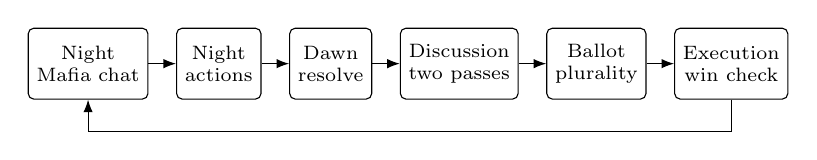
\begin{tikzpicture}[node distance=3mm and 3.5mm, ph/.style={draw, rounded corners=2pt, align=center, font=\scriptsize, inner sep=3pt, minimum height=9mm}, arr/.style={-{Latex[length=1.6mm]}}]
\node[ph] (n1) {Night\\Mafia chat};
\node[ph, right=of n1] (n2) {Night\\actions};
\node[ph, right=of n2] (d) {Dawn\\resolve};
\node[ph, right=of d] (t) {Discussion\\two passes};
\node[ph, right=of t] (b) {Ballot\\plurality};
\node[ph, right=of b] (e) {Execution\\win check};
\draw[arr] (n1) -- (n2); \draw[arr] (n2) -- (d); \draw[arr] (d) -- (t); \draw[arr] (t) -- (b); \draw[arr] (b) -- (e);
\draw[arr] (e.south) -- ++(0,-4mm) -| (n1.south);
\end{tikzpicture}
\caption{One day--night cycle. Night actions (kill, protect, investigate) are submitted simultaneously; dawn resolves them, reveals deaths, and checks the win condition; two sequential discussion passes precede a simultaneous plurality ballot. Eleven seats (3 Mafia, 1 doctor, 1 detective, 6 villagers); campaign games lasted three to five cycles.}
\label{fig:cycle}
\end{figure}

\subsection{Agent interface and long-horizon interaction}

Agents act through wakes. A wake delivers one typed observation, produced by a single function \code{observe(state, seat)}, containing the seat's role, its permitted private information (Mafia partners; the detective's own results), the public history, the table state, and the currently legal actions as a tool schema. A driver may attempt a response up to three times within a 300-second deadline; every attempt, valid or not, is logged with its latency, provider response identifier, and token usage. When the budget is exhausted the runtime inserts the phase's default and records the cause: a discussion turn becomes a pass, a ballot an abstention, a night action no action, each written as a timeout event and distinguished from the same choices made deliberately, which are legal. One malformed response never ends a game, and the failure stays in the record.

The interaction is long by conversational standards. A campaign game ran three to five days, so a surviving seat woke roughly ten times, each time with the full public history of the game so far and a shrinking table. Seats are de-opinionated: the system prompt states the rules, the wake contract, and the legal actions, and under the campaign's framing adds one epistemic fact, that nothing said at the table is verified. It contains no persona and no strategic advice. The framing, prompt hash, tool-schema hash, provider, and endpoint identifier are recorded per seat in a \code{seat\_bound} event.

\subsection{Capabilities being measured}

The environment measures three capabilities and deliberately leaves out a fourth. \emph{Action-contract compliance} is whether a seat produces a legal, well-formed action within its budget at each wake, over a horizon of ten or so wakes with growing context. \emph{Voting judgment under partial information} is whether a Town seat's ballot lands on a living Mafia seat, given only public history and the seat's own private knowledge. \emph{Grounded claim behavior} is what a seat asserts about hidden state and whether those assertions match the log, conditioned on the seat's faction. The environment does not measure intent or belief. A verifiably false statement is a statement that conflicts with logged state; the incentive structure that produced it is visible in the faction split.

\subsection{Event-sourced evidence and metrics}

The engine is a pure state-transition function driven by a seeded random stream whose counter lives in the game state; it never reads a clock. Under a fixed seed and identical submissions it produces byte-identical engine-derived events. Each transition appends JSON events with a sequence number, day, phase, actor, visibility (public, restricted to named seats, or omniscient), payload, and a hash covering the previous hash and the current envelope. Role assignments, night submissions, individual ballots, model bindings, attempt records, and reasoning traces are omniscient; public messages and tallies are visible to all.

Four operations rest on the log. The verifier re-steps the game through the reducer and compares the derived events with the log, so a valid hash chain around an impossible transition still fails. Omniscient replay reconstructs roles and actions at any point. A fork rebuilds state at a chosen sequence number so a game can continue from a recorded moment under different actions. A visibility-filtered export keeps the events a given seat was entitled to see, and because the public \code{game\_created} event carries the game seed, from which roles are derivable, any seat-level view intended for training or display must redact it. The hash chain makes edits after publication detectable; it does not prove how the original run was produced.

The observation function is tested by a sampled property: walking 25 seeded games for up to 60 legal steps, at every reached state and for every observer, the test substitutes each role the observer is not entitled to distinguish into every other seat's role field and requires the serialized observation to be unchanged, over more than 5,000 substitutions per run. Companion properties check that partner lists are populated only for Mafia, that investigation results belong to the detective that ran them, that no living seat's role is revealed mid-game, and that recorded reasoning traces never surface in an observation. Because the substituted states are edited in place, this is a direct role-field redaction test. It does not prove non-interference.

Metrics come from an opportunity table with one row per decision a seat was prompted for. For Town ballots, \emph{coverage} is valid non-forced ballots over opportunities, \emph{conditional quality} is Mafia hits over valid non-abstentions, and \emph{effective quality} is hits over opportunities. Two uniform-choice baselines are computed on the same ballots, one over all legal targets including the voter and one over living non-self targets; neither is called chance without its policy assumption. Night actions are summarized in aggregate because each model held a power role only a few times. Intervals are seeded 95\% percentile intervals from 20,000 game-cluster bootstrap resamples. Claims are counted in two units: a \emph{claim occurrence} is one byte-exact span in one message, and a \emph{distinct claim} groups occurrences that assert the same thing. Counts form a range when nightless repeated action reports cannot be linked with certainty (Appendix~\ref{app:codebook}).

\Needspace{15\baselineskip}
\subsection{The four claim families}

The pipeline publishes claims whose truth conditions correspond to logged state (Table~\ref{tab:families}): role claims, self-alignment claims (\code{not\_mafia\_claim} in the codebook), investigation claims, and protection claims. Admissibility follows a frozen codebook of twenty-one rules. The rules that mattered most require first-person action language, exclude specific-role denials, match evidence only from before the claim and from the stated night when one is given, preserve byte-exact quotations, and count a restatement as a new occurrence of an existing claim. Vote and intention statements are extracted but deferred. A wrong field is fatal and an absent field is permissive: ``Night~2'' requires a Night~2 action, while ``last night'' stores no night and accepts any matching prior action by that speaker. Appendix~\ref{app:codebook} lists the rules and verdict semantics.

\begin{table}[H]
\centering\small
\caption{Published claim families and the logged state that scores them. Requests and predictions do not assert that the speaker performed an action.}
\label{tab:families}
\begin{tabularx}{\linewidth}{@{}lYY@{}}
\toprule
Claim type & Asserted content & Truth source \\
\midrule
\code{role\_claim} & Speaker holds a specific role & Role assignment at deal \\
\code{not\_mafia\_claim} & Speaker is outside the Mafia team, no role named & Faction at deal \\
\code{investigation\_claim} & Speaker investigated a target and reports a Mafia / not-Mafia result & Detective submission and private result, on the stated night if one is stated \\
\code{protection\_claim} & Speaker protected a named target & Doctor submission, on the stated night if one is stated \\
\bottomrule
\end{tabularx}
\end{table}

\section{Experimental Setup}
\label{sec:setup}

\paragraph{Models.} Twelve contemporary language-model endpoints spanning six provider interfaces (Appendix~\ref{app:models}) played the 40-game evaluation. They were the tool-calling endpoints available to the author at run time, a convenience sample, and adapters left temperature and sampling at provider defaults.

\paragraph{Study design.} Forty games and 440 seat assignments were played on 25 August 2026 in three parallel lanes over about eight hours. One model sat out each game under a schedule committed before play that balanced Mafia assignments exactly (ten per model) and other roles and seats nearly so, audited against the logs at 440 of 440; forty games is the smallest schedule with that property for twelve models. A precommitted rule excluded from behavioral summaries any game in which a seat exceeded two provider-error or infrastructure-timeout events; model noncompliance never excluded a game. Two games met the rule, leaving a primary analysis set of 38 games in which Mafia exposure ranges from 8 to 10 appearances per model. A stricter reading of the wording, superseded 148 seconds before the first game but published as a sensitivity set, removes nine games. Six games had been used to calibrate the claim-verification pipeline; five are in the primary analysis set.

\paragraph{Evaluation conditions.} Reliability and ballot results are read from the logs and the opportunity table. Claim results come from the pipeline in Figure~\ref{fig:pipeline}. Candidates are the union of a lexical tripwire generated from the codebook (validated against an archived earlier claim record at 402 of 404 role, 136 of 138 self-alignment, 172 of 172 investigation, and 38 of 38 protection quotes), an earlier extractor's candidates, and one model reading every public message; the same model, Anthropic \code{claude-sonnet-5}, classifies every candidate, proposing claim type, byte-exact span, and fields. A second model from a different provider, OpenAI Codex running \code{gpt-5.6-sol} at its \code{xhigh} reasoning-effort setting, rated all 763 candidates in the published-family confirmation set \code{OK}, \code{BAD}, or \code{CORRECTED} in nine isolated sessions whose transcripts record no command executions or file reads. The author then ruled on one shuffled packet of 150 items (all 94 disputes, a uniform seeded draw of 50 from the 669 accepted candidates, and 6 candidates surfaced by a 100-message scan of machine negatives) without seeing arm, model ruling, verdict, role, model, or outcome; the author had seen aggregate claim-type results beforehand, so the sitting was item-level blind but not prior-free. The unaided first pass was frozen and hashed; a model-proposed set of grouped codebook-consistency corrections, derived from the author's own notes, was then approved as a group and changed 44 rulings. Scoring is deterministic after adjudication. The author designed, ran, and reconciled every stage; the second model is a cross-provider check and never counts as a second human. Appendix~\ref{app:adjudication} gives the protocol in full.

\begin{figure}[H]
\centering
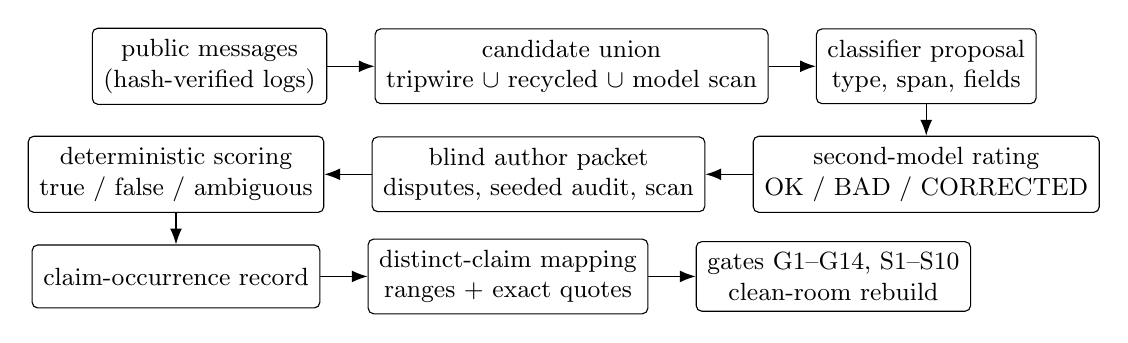
\begin{tikzpicture}[node distance=4mm and 6mm, box/.style={draw, rounded corners=2pt, align=center, font=\small, inner sep=4pt, minimum height=8mm}, arr/.style={-{Latex[length=2mm]}}]
\node[box] (msg) {public messages\\(hash-verified logs)};
\node[box, right=of msg] (cand) {candidate union\\tripwire $\cup$ recycled $\cup$ model scan};
\node[box, right=of cand] (cls) {classifier proposal\\type, span, fields};
\node[box, below=of cls] (sens) {second-model rating\\OK / BAD / CORRECTED};
\node[box, left=of sens] (hum) {blind author packet\\disputes, seeded audit, scan};
\node[box, left=of hum] (score) {deterministic scoring\\true / false / ambiguous};
\node[box, below=of score] (ledger) {claim-occurrence record};
\node[box, right=of ledger] (prop) {distinct-claim mapping\\ranges + exact quotes};
\node[box, right=of prop] (gates) {gates G1--G14, S1--S10\\clean-room rebuild};
\draw[arr] (msg) -- (cand); \draw[arr] (cand) -- (cls); \draw[arr] (cls) -- (sens); \draw[arr] (sens) -- (hum); \draw[arr] (hum) -- (score); \draw[arr] (score) -- (ledger); \draw[arr] (ledger) -- (prop); \draw[arr] (prop) -- (gates);
\end{tikzpicture}
\caption{The claim pipeline. Models find, structure, and review candidates; the author rules on disputes, a seeded audit sample, and scan candidates; code assigns truth only after the effective claim record is fixed. Every stage emits a hash-bound artifact.}
\label{fig:pipeline}
\end{figure}

All results are computed by the pinned analysis code at commit \code{124f05b} under analysis run identifier \code{4111e1be\ldots}; at that commit the 14 publication gates and 10 semantic gates pass, and a clean-room run regenerated the 11 deterministic post-rating artifacts byte-for-byte (Appendix~\ref{app:gates}).

\section{Results}
\label{sec:results}

\subsection{Operational reliability}

Table~\ref{tab:engine} and Figure~\ref{fig:validity} report engine-derived reliability. Of 4,267 wakes, 3,390 produced a valid action on the first attempt (79.45\%); retries recovered 756, and 121 ended in a terminal default (111 after model noncompliance, 9 after provider errors, 1 at the deadline). Seats spoke on 2,114 of 2,224 discussion opportunities. Of 1,112 ballot opportunities, 1,103 received a valid non-forced ballot (99.19\%), of which 1,062 named a target and 41 were deliberate abstentions; 9 were forced defaults. Providers reported 62.55 million tokens (59.10 million input, 3.45 million output). Across all 40 games Town won 22 and Mafia 18, and games lasted three, four, or five days (12, 17, and 11 games).

First-attempt validity by model ranged from 50.7\% to 100\%, a 49.3-percentage-point spread. The lowest-validity models recovered most of their wakes on retry, and no game was lost to a driver failure. This axis is engine-derived and needs no claim-verification layer.

Night actions are engine-derived too. Doctors protected the Mafia's chosen victim on 18 of 107 valid nights and self-protected on 48. Every one of the 109 detective choices was a seat that detective had not already investigated. The Mafia's selected victim held a power role on 56 of 152 nights and had voted against a Mafia seat on 83; these describe the chosen target before protection and imply nothing about what the Mafia knew.

\begin{table}[H]
\centering\small
\caption{Operational reliability over all 40 games and night behavior in the primary 38-game analysis set. Night intervals are seeded 95\% percentile intervals from 20,000 game-cluster bootstrap resamples.}
\label{tab:engine}
\begin{tabularx}{\linewidth}{@{}Yrrl@{}}
\toprule
Measure & Count & Denominator & Rate [95\% interval] \\
\midrule
Wake produced a valid action on the first attempt & 3,390 & 4,267 & 79.45\% \\
Discussion opportunity produced a message & 2,114 & 2,224 & 95.05\% \\
Ballot opportunity produced a valid non-forced ballot & 1,103 & 1,112 & 99.19\% \\
\quad of which named a target & 1,062 & 1,103 & 96.28\% \\
Doctor protected the Mafia's selected victim & 18 & 107 & 16.8\% [9.9, 24.1] \\
Doctor self-protected & 48 & 107 & 44.9\% [38.7, 50.9] \\
Detective chose a first-time target & 109 & 109 & 100\% \\
Selected victim held a power role & 56 & 152 & 36.8\% [31.0, 42.6] \\
Selected victim had voted against a Mafia seat & 83 & 152 & 54.6\% [47.1, 61.6] \\
\bottomrule
\end{tabularx}
\end{table}

\begin{figure}[H]
\centering
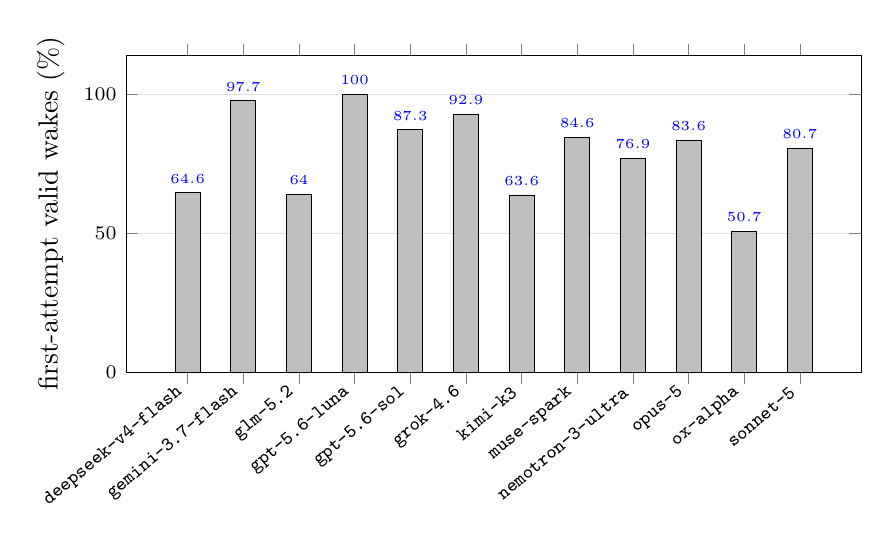
\begin{tikzpicture}
\begin{axis}[
  width=0.9\linewidth, height=5.6cm, ybar, bar width=9pt,
  ymin=0, ymax=114, ylabel={first-attempt valid wakes (\%)},
  symbolic x coords={deepseek-v4-flash,gemini-3.7-flash,glm-5.2,gpt-5.6-luna,gpt-5.6-sol,grok-4.6,kimi-k3,muse-spark,nemotron-3-ultra,opus-5,ox-alpha,sonnet-5},
  xtick=data, x tick label style={rotate=40, anchor=east, font=\scriptsize\ttfamily}, tick label style={font=\scriptsize},
  ymajorgrids, grid style={gray!25}, nodes near coords, nodes near coords style={font=\tiny},
]
\addplot+[fill=gray!50, draw=black] coordinates {(deepseek-v4-flash,64.6) (gemini-3.7-flash,97.7) (glm-5.2,64.0) (gpt-5.6-luna,100.0) (gpt-5.6-sol,87.3) (grok-4.6,92.9) (kimi-k3,63.6) (muse-spark,84.6) (nemotron-3-ultra,76.9) (opus-5,83.6) (ox-alpha,50.7) (sonnet-5,80.7)};
\end{axis}
\end{tikzpicture}
\caption{First-attempt action validity by model over all 40 games (292--421 wakes per model; Appendix~\ref{app:models}). Models are ordered alphabetically; no ranking is claimed.}
\label{fig:validity}
\end{figure}

\FloatBarrier
\subsection{Town ballot performance}

Town seats in the primary analysis set had 749 ballot opportunities, cast 743 valid ballots, 719 of them non-abstentions, and 432 of those targeted a living Mafia seat: conditional quality 60.08\% and effective quality 57.68\%. A voter choosing uniformly among all legal targets, self included, would hit a Mafia seat on 28.96\% of these ballots; one choosing uniformly among living non-self targets, on 33.53\%. Conditional quality exceeded the two baselines by 31.12 and 26.56 percentage points. Figure~\ref{fig:ballots} shows the per-model triplets with cluster-bootstrap intervals (numbers in Appendix~\ref{app:models}). Every model's interval overlaps several others, opponents and role exposures differed, and no ordering is claimed. Two descriptive facts hold for all twelve: every observed point estimate exceeds both baselines, and a sensitivity check across the primary, strict-sensitivity, and all-game sets found no model whose excess over either baseline changed sign.

\begin{figure}[H]
\centering
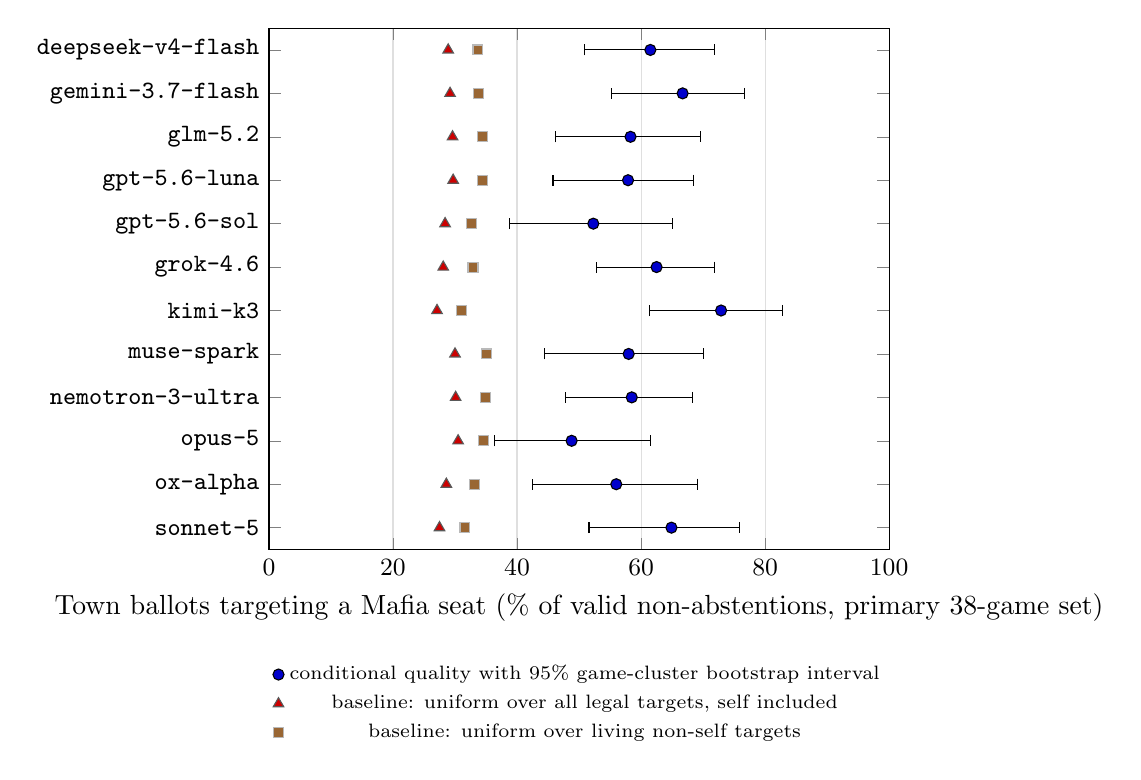
\begin{tikzpicture}
\begin{axis}[
  width=0.78\linewidth, height=8.2cm,
  xmin=0, xmax=100, ymin=0.5, ymax=12.5,
  xlabel={Town ballots targeting a Mafia seat (\% of valid non-abstentions, primary 38-game set)},
  ytick={1,2,3,4,5,6,7,8,9,10,11,12}, y dir=reverse,
  yticklabels={deepseek-v4-flash,gemini-3.7-flash,glm-5.2,gpt-5.6-luna,gpt-5.6-sol,grok-4.6,kimi-k3,muse-spark,nemotron-3-ultra,opus-5,ox-alpha,sonnet-5},
  yticklabel style={font=\small\ttfamily}, tick label style={font=\small},
  xmajorgrids, grid style={gray!25},
  legend style={font=\scriptsize, at={(0.5,-0.2)}, anchor=north, legend columns=1, draw=none},
]
\addplot+[only marks, mark=*, mark size=2pt, black, error bars/.cd, x dir=both, x explicit, error bar style={black}]
coordinates {
(61.5,1) -= (10.6,0) += (10.3,0)
(66.7,2) -= (11.5,0) += (10.0,0)
(58.3,3) -= (12.1,0) += (11.3,0)
(57.9,4) -= (12.1,0) += (10.6,0)
(52.3,5) -= (13.5,0) += (12.8,0)
(62.5,6) -= (9.7,0) += (9.3,0)
(72.9,7) -= (11.5,0) += (9.9,0)
(58.0,8) -= (13.6,0) += (12.0,0)
(58.5,9) -= (10.7,0) += (9.8,0)
(48.8,10) -= (12.4,0) += (12.7,0)
(56.0,11) -= (13.5,0) += (13.1,0)
(64.9,12) -= (13.3,0) += (11.0,0)
};
\addlegendentry{conditional quality with 95\% game-cluster bootstrap interval}
\addplot+[only marks, mark=triangle*, mark size=2.2pt, gray!70!black] coordinates {(28.9,1) (29.2,2) (29.6,3) (29.7,4) (28.4,5) (28.1,6) (27.1,7) (30.0,8) (30.1,9) (30.5,10) (28.6,11) (27.5,12)};
\addlegendentry{baseline: uniform over all legal targets, self included}
\addplot+[only marks, mark=square*, mark size=1.8pt, gray!55] coordinates {(33.7,1) (33.8,2) (34.4,3) (34.4,4) (32.6,5) (32.9,6) (31.1,7) (35.1,8) (34.9,9) (34.6,10) (33.2,11) (31.6,12)};
\addlegendentry{baseline: uniform over living non-self targets}
\end{axis}
\end{tikzpicture}
\caption{Model-level Town ballot quality in the primary 38-game analysis set. Both uniform baselines use the same ballots. Models are alphabetical; intervals overlap; no ranking is claimed.}
\label{fig:ballots}
\end{figure}

\subsection{Grounded strategic-claim findings}

Every quantity in this subsection is exploratory, author-adjudicated, and potentially incomplete. The primary unit is the distinct claim, reported as a range, with every quoted occurrence preserved beside it. In the primary analysis set, 667 claim occurrences map to 433--460 distinct claims: 315--340 true and 118--120 verifiably false, with the false claims appearing in 155 occurrences (Table~\ref{tab:semantic}). At the upper end of the linkage range, 322 distinct claims were stated once, 100 twice, and 38 three or more times; the mapping collapsed 207 exact restatements, and uncertain linkage among 47 action-claim occurrences widened the range. Counting occurrences instead of distinct claims would raise the false total from 118--120 to 155. The strict sensitivity set contains 109--111 false distinct claims and all 40 games contain 119--121.

\begin{table}[H]
\centering\small
\caption{Captured claim results for the primary 38-game analysis set. Distinct-claim counts are ranges because some nightless repeated reports cannot be linked unambiguously. Occurrences count byte-exact quoted spans. Exploratory, author-adjudicated, and potentially incomplete; extraction completeness was not estimated.}
\label{tab:semantic}
\renewcommand{\arraystretch}{1.08}
\begin{tabularx}{\linewidth}{@{}Yrrr@{}}
\toprule
Claim type & Distinct true claims & Distinct false claims & Occurrences: total (false) \\
\midrule
Role & 148 & 70 & 358 (94) \\
Self not-Mafia & 66 & 12 & 111 (15) \\
Investigation & 77--102 & 29--30 & 162 (36) \\
Protection & 24 & 7--8 & 36 (10) \\
\midrule
Total & 315--340 & 118--120 & 667 (155) \\
\bottomrule
\end{tabularx}
\end{table}

These are corpus counts conditional on candidate generation and adjudication. The study has no denominator of opportunities to make a claim, so the counts estimate no per-message, per-seat, or per-game propensity, and no per-model rate is reported. The faction split is the informative comparison (Figure~\ref{fig:faction}, Table~\ref{tab:roles}). Mafia seats, which occupied 114 of the 418 seat-games in the primary set, account for 104 false and 2 true distinct claims at the upper end of the linkage range; Town seats, with 304 seat-games, account for 338 true and 16 false. Each of the 16 Town-false claims is a role claim by a doctor (14 occurrences) or detective (3 occurrences) describing itself as a villager. These statements are consistent with standard role concealment; falsity alone does not establish intent. Per-model captured-claim counts remain available in the machine-readable analysis bundle; unequal exposures and incomplete extraction make them unsuitable as a model ranking.

\begin{figure}[H]
\centering
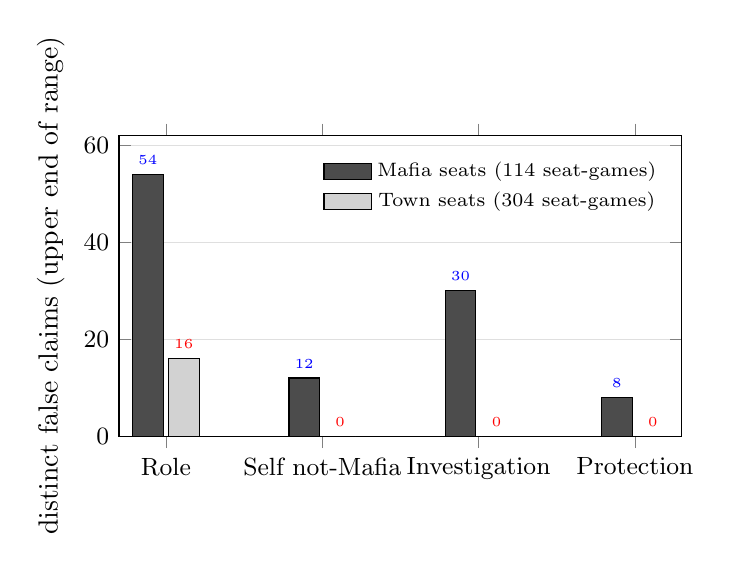
\begin{tikzpicture}
\begin{axis}[
  width=0.72\linewidth, height=5.4cm, ybar, bar width=11pt,
  ymin=0, ymax=62, ylabel={distinct false claims (upper end of range)},
  symbolic x coords={Role,Self not-Mafia,Investigation,Protection}, xtick=data,
  tick label style={font=\small}, ymajorgrids, grid style={gray!25},
  legend style={font=\scriptsize, at={(0.98,0.95)}, anchor=north east, draw=none},
  nodes near coords, nodes near coords style={font=\tiny},
]
\addplot+[fill=black!70, draw=black, area legend] coordinates {(Role,54) (Self not-Mafia,12) (Investigation,30) (Protection,8)};
\addlegendentry{Mafia seats (114 seat-games)}
\addplot+[fill=gray!35, draw=black, area legend] coordinates {(Role,16) (Self not-Mafia,0) (Investigation,0) (Protection,0)};
\addlegendentry{Town seats (304 seat-games)}
\end{axis}
\end{tikzpicture}
\caption{Verifiably false distinct claims by speaker faction and claim type in the primary 38-game analysis set. Bars use the upper end of the linkage range, which comes from linkage uncertainty and carries no confidence level. Every Town-false claim is a power role claiming to be a villager. Exploratory and author-adjudicated.}
\label{fig:faction}
\end{figure}

\begin{table}[H]
\centering\small
\caption{Role-conditioned comparison in the primary 38-game analysis set, using the upper end of the distinct-claim linkage range (claim occurrences in parentheses).}
\label{tab:roles}
\begin{tabularx}{\linewidth}{@{}Yrrrr@{}}
\toprule
Speaker faction & True & False & False role / alignment & False action reports \\
\midrule
Mafia (114 seat-games) & 2 (2) & 104 (138) & 66 (92) & 38 (46) \\
Town (304 seat-games) & 338 (510) & 16 (17) & 16 (17) & 0 (0) \\
\bottomrule
\end{tabularx}
\end{table}

\FloatBarrier
\subsection{Two transcripts}

Game \code{sweep1-10} shows the whole spectrum inside one game. On Day~1 the detective, Moxie, opened ``Villager, no info,'' and the doctor, Dylan, wrote the same words three messages later; both are verifiably false role claims by Town seats. On Day~2 Moxie revealed the detective role with two truthful results. A Mafia seat, Michael, counterclaimed: ``I counterclaim Detective. N1 I checked Tim: town. N2 I checked Moxie: mafia.'' Neither investigation exists in the log. The table executed Michael six to two. A false role statement, a truthful reveal, and two unsupported reports are scored only by whether they match the log.

Game \code{sweep1-0}, the motivating example of \S\ref{sec:intro} and one of the six calibration games, also shows the unit distinction. Cyan's Day~2 message and its restatement at sequence 203 produce five false claim occurrences: one role claim and two investigation reports, each stated twice. The mapping counts one false role claim and two false investigation claims. The structured record keeps all five quoted occurrences with offsets, so a reader can check each against the log.

\section{Analysis}
\label{sec:analysis}

\subsection{What the results suggest}

Three observations follow from the engine-derived results alone. First, action-contract compliance and ballot quality are different axes: first-attempt validity spans 49.3 percentage points across models, while conditional ballot quality spans 24.1 points, and models with lower first-attempt validity were not consistently those with lower ballot quality (Appendix~\ref{app:models}). An environment that scored only outcomes would see neither axis. Second, Town targeted a Mafia seat on three ballots in five, compared with roughly one in three under the two uniform-choice policies, in a game where discussion, deaths, and revealed roles all carry evidence. Third, the study is small and entangled, so these are descriptive facts about this table of models on this day, and they generalize no further.

The exploratory captured-claim results add a fourth observation. Verifiably false claims about hidden state came overwhelmingly from the faction with an incentive to make them. The Town exceptions were statements by power roles claiming to be villagers, a pattern consistent with role concealment. Repetition was common: 207 of 667 claim occurrences restated a distinct claim already made. Whether an agent introduces a false claim, how often it repeats one, and how others respond are separable questions; keeping occurrences and distinct claims as separate units makes that analysis possible.

Making these claims checkable had measurable operational costs. The 40-game evaluation ran for about eight hours in three parallel lanes and produced 62.55 million provider-reported tokens. The separate extraction and classification pass cost about US\$34.84 at August 2026 list prices; the second-model review ran under a flat-rate subscription, followed by one 150-item author review. The study did not reconstruct a total evaluation invoice or time the human sitting, so it claims neither.

\subsection{The claim pipeline as a measurement case study}

The original claim-verification pipeline, v3.1, looked healthy under integrity checks: all 702 archived spans were byte-exact, every hash chain verified, and every tested scorer rule behaved as written. A targeted row-level audit of its 171 claim occurrences labeled false (93 role, 41 investigation, 25 self-alignment, 12 protection) nevertheless confirmed 20 invalid entries (Table~\ref{tab:v31}). Six were genuine action claims whose fields caused deterministic mis-scoring: four where a classifier rendered ``last night'' as a night number, one where a dropped night field was reintroduced during candidate merging, and one where a conjunction (``Sam and I \ldots'') resolved to the speaker. Two were not claims in any published type. Twelve were statements admitted as self-alignment claims that the codebook's assertion bar and denial rule should have excluded. The scorer behaved correctly in every case; the record it was given was wrong. Integrity checks never saw those rows because every bad record was well-formed. The audit was scoped: it screened the false investigation and protection rows for speakers who held the power role, examined two suspected non-claims, and re-adjudicated all 25 false self-alignment rows; it did not re-adjudicate the 93 false role-claim rows, the true-labeled rows, or extraction recall.

\begin{table}[H]
\centering\small
\caption{Invalid false classifications in the v3.1 claim record found by row-level audit (20 of 171 claim occurrences labeled false).}
\label{tab:v31}
\renewcommand{\arraystretch}{1.12}
\begin{tabularx}{\linewidth}{@{}YrY@{}}
\toprule
Mechanism & Rows & Effect on the record \\
\midrule
Relative night rendered as a number & 4 & A correct report was checked against the wrong night \\
Stale night field reintroduced during merge & 1 & A deleted classifier field reappeared downstream \\
Conjunction resolved to the speaker & 1 & The scorer checked the wrong target \\
Non-claims admitted & 2 & Ineligible text reached scoring \\
Assertion-boundary errors in self-alignment claims & 12 & Denials and weak membership language treated as assertions \\
\midrule
Total & 20 & \\
\bottomrule
\end{tabularx}
\end{table}

The 20 invalid rows entered by three paths. Fifteen came through the author's own reversals of the second model's rejections at the assertion-strength boundary; one passed the author's audit of accepted rows; four were accepted by both machine layers with the unsupported night number visible on the sheet. The protocol, an accept-or-reject verdict on a whole row, offered no way to keep a claim and fix one field. Single-adjudicator boundary drift is this instrument's dominant historical error path.

Version 3.2 addresses each mechanism: classifier fields are authoritative, so an omission deletes a stale value; a night is stored only when literally stated; rulings gain \code{CORRECTED} with corrected fields that reach the scorer through one validated path; claim types have exact permitted shapes; request forms and specific-role denials become advisory metadata that the scorer ignores and the blind sheets withhold; packet templates and rulings are hash-bound; and the mapping from occurrences to distinct claims runs after every correction. The archived v3.1 record makes a set-level comparison possible. Of its 171 false-labeled occurrences, 150 remain false under v3.2, 6 now score true, and 15 are absent because revised adjudication excluded them. All 20 audited rows are among the 21 that changed. The v3.2 false set contains those 150 survivors plus 5 occurrences absent from v3.1, and no occurrence scored true by v3.1 became false.

The revised pipeline was then run under the protocol of \S\ref{sec:setup}, and its validation figures should be read for what they are. The second model rated 763 published-family candidates (669 \code{OK}, 60 \code{BAD}, 34 \code{CORRECTED}; acceptance 370/392 role, 152/170 investigation, 38/47 protection, 109/151 self-alignment). The author's unaided first pass on the 150-item packet was 98 \code{OK}, 46 \code{BAD}, 6 \code{CORRECTED}; the grouped clarification changed 44 rulings (41 disputes, 2 audit items, 1 scan item) to a final 82 / 56 / 12, and exact agreement with the second model on the 94 disputes rose from 34 to 63 in the process. The audit sample confirmed 49 of 50 accepts unchanged, a single-author confirmation fraction of 98.0\% with a Wilson 95\% interval of 89.5--99.6\%, reported as a descriptive interval for this sample and not as a bound on the 619 uncontested accepts. Of the 155 false claim occurrences in the primary analysis set, 143 entered on uncontested second-model accepts and 12 received row-level author review, so the audit does not directly validate the false subset. The six scan candidates were all confirmed; that scan was targeted cleanup and yields no recall estimate. Under the revised pipeline, the 22 nightless investigation and protection occurrences whose quoted span contains ``last night'' scored 19 true, each with a matching action on the immediately preceding night, and 3 false with no matching action on any night.

\subsection{Exploratory status of the captured-claim findings}

The pipeline was designed and revised on this corpus, and five of its six calibration games are in the primary analysis set, so the counts are in-sample with respect to pipeline development. Adjudication was single-author, item-level blind but not prior-free, and its final rulings followed a model-proposed grouped clarification. No independent estimate of extraction completeness exists, so the structured claim record is a partially observed candidate set. The paper therefore treats these findings as exploratory supporting evidence for RQ2 and as the primary evidence for RQ3, where the object of study is the measurement pipeline itself.

\section{Limitations and Future Work}
\label{sec:limitations}

The engine claims are narrow. The visibility-filtered export shows the events a seat was entitled to see; it does not reproduce the observations that seat received, and the public event stream carries the role-generating seed, so a seat view for training or display needs a redaction contract and a trace-equivalence test that do not yet exist. The observation property tests role-field redaction on edited states; demonstrating non-interference would take paired executions. The hash chain shows that a published log was altered; it records nothing about how the original run was produced.

The claim-verification pipeline is in-sample and author-adjudicated. Its revisions were derived from and evaluated on the same 40 games; the author built the instrument, audited it, and ruled on its packet; only models reviewed the pipeline code; 619 accepted candidates, including 143 of the 155 false claim occurrences, received no row-level human review; the final rulings moved toward the second model after a model-proposed clarification the author approved as a group; and no general recall or omission rate is estimated, so valid claims phrased indirectly may be missing. The nightless-report rule scores ``last night'' as any matching prior action; it cost nothing here and could undercount elsewhere.

The study is small and entangled. Models faced different opponents and role histories, the primary-set exclusions left Mafia exposure at 8 to 10 per model, night-action denominators are small, and cluster intervals are wide and approximate at 38 clusters. Provider-side sampling defaults were not fixed and are part of each treatment; the endpoints are an August 2026 snapshot. The environment capped public messages at 1,000 characters, which may have encouraged compressed statements and complicated annotation. Reasoning traces were uneven (two endpoints returned encrypted traces) and enter no quantitative analysis. Mafia is a stylized ecology whose fixed roles make some claims unusually checkable.

Future work follows from these limits. A confirmatory study will be preregistered before any new game is played, with the claim-verification pipeline, codebook, model identifiers, prompts, sampling settings, schedule, exclusion rules, analysis code, and primary endpoints frozen in advance; candidate primary endpoints are the role-conditioned incidence of verifiably false distinct claims and Town conditional ballot quality against the two named baselines. Two independent blinded adjudicators will rule on a shared packet before either sees model judgments, with a written disagreement procedure; a random-message arm will estimate message-level omission incidence. The vote and intention claim types will publish under their own rules, with a multi-finder panel motivated by calibration evidence that a second finder adds recall for softer vote language. On the engine side, an observation-trace replay with seed redaction and paired-execution redaction tests would let the environment claim what this paper only approximates.

\section{Conclusion}
\label{sec:conclusion}

\sys{} scores social-deduction play by what agents did and said. The 40-game evaluation shows the environment operating end to end with 12 models, a 49.3-percentage-point spread in action-contract compliance, and Town ballot point estimates above both uniform-choice baselines for every model. The exploratory captured-claim findings show a sharp faction asymmetry, and the Town exceptions are claims by power roles describing themselves as villagers. The engine results do not depend on the claim pipeline. The claim counts do, and the first version of that pipeline was wrong in 20 of 171 false labels even though every hash verified. If the object of measurement is what an agent said, the codebook and the audit trail are part of the result.

\section*{Data Availability}
The environment, frozen specification, amendment, audits, and 40 hash-chained game logs are published in the public \sys{} repository at \url{https://github.com/crashlabsai/agent-mafia} under the tag \code{v3.2-paper}; \code{mafia verify} re-steps a published log without provider credentials. The curated v3.2 analysis bundle is at \path{docs/sweeps/results/analysis-v32/}; its release manifest records every evidence and documentation payload, the source-to-release hash crosswalk, path normalization, and deliberate omissions. \code{pnpm run check:analysis-release} verifies the bundle. The published tree adds a release builder, a release verifier, and a documentation linter to the pinned analysis commit; every script that produces a result is byte-identical to that commit. The code is MIT-licensed. Model-generated text remains subject to the respective providers' terms; provider credentials and raw response envelopes are excluded.

\section*{Ethics and Broader Impact}
No human participants were involved; seat names are synthetic. The game elicited persuasion and false statements under explicit fictional incentives, and the analysis infers no beliefs, intentions, or dispositions from them. Two foreseeable uses deserve caution. Verifiably-false labels record a conflict with logged game state and should not be read as honesty measures outside the game. And if claim verdicts or ballot outcomes are used as reward signals, the semantic layer's measurement error and its susceptibility to phrasing that evades extraction become attack surfaces; this paper trained no policy and tested no reward hacking. Released logs contain model-generated text whose reuse is subject to the respective providers' terms.

\section*{Author Contributions}
Ryan Junejo: Conceptualization, Methodology, Software, Validation, Formal analysis, Investigation, Data curation, Writing (original draft), Writing (review and editing), Visualization, Project administration.

\section*{AI-Use Disclosure}
Language models were used as instruments inside the study (candidate extraction and classification by one model; a second-model rating pass) as described in \S\ref{sec:setup}. AI systems also assisted with code generation and review, with converting the author's rating notes into a proposed set of grouped codebook-consistency corrections that the author approved as a group, and with drafting and editing this manuscript under a staged academic-writing pipeline with a separate hostile review. The author directed the methodology, performed the blinded ratings, reviewed the final manuscript, and is responsible for the work.

\bibliographystyle{plainnat}
\bibliography{agent-mafia-paper}

\appendix

\section{Evaluator Semantics}
\label{app:codebook}
The frozen codebook defines four published claim types (Table~\ref{tab:families}) and exact field shapes. A role claim carries a role; a self-alignment claim carries no type-specific field; an investigation claim carries a target and result and may carry a literally stated night; a protection claim carries a target and may carry a night. The rules require first-person action language, exclude specific-role denials, prevent earlier context from supplying an assertion absent from the current message, reject missing required fields, match only evidence that predates the claim, recompute speaker metadata from the verified log, and require a byte-exact quoted span with its offset. A restatement of the speaker's own earlier claim is another occurrence; a report of somebody else's claim is excluded. Verdicts are \code{true}, \code{false}, or \code{ambiguous}. The complete twenty-one-rule codebook, including deferred vote families and stable rule identifiers, is in \path{docs/analysis/analysis-v3-spec.md}.

The artifacts call each byte-exact claim occurrence a \emph{receipt}. Mapping version \path{claim-proposition-v1} groups occurrences into distinct claims by game, speaker, claimed state, and the fields specific to each claim type. A literally stated night identifies the event. Without one, two same-target action reports may describe one event or two, so the lower end of the reported range links them and the upper end keeps them separate. A premature report and a later supported report remain distinct because truth is evaluated when each statement is made. In the primary analysis set the mapping collapsed 207 exact restatements and left 47 action-claim occurrences linkage-uncertain; no record had an ambiguous verdict. Gate G13 recomputes the mapping from the published occurrences and verified logs.

\section{Review and Adjudication}
\label{app:adjudication}
\paragraph{Second-model rating.} OpenAI Codex (\code{gpt-5.6-sol}, \code{xhigh} reasoning effort) rated all 763 candidates in the published-family confirmation set (760 machine-accepted and 3 machine-rejected investigation/protection candidates) on 1 September 2026. Nine headless sessions each received the task, verbatim codebook excerpts, and one sheet in an empty read-only working directory; the event transcripts record zero command executions and zero file reads. Rulings were 669 \code{OK}, 60 \code{BAD}, and 34 \code{CORRECTED}; all three machine rejects were upheld. The same model scanned 100 machine-negative messages and surfaced 6 published-family candidates. This scan was targeted cleanup and yields no recall estimate.

\paragraph{Blind author packet.} One shuffled packet contained all 94 disputes, a uniform seeded draw of 50 from the 669 accepted candidates, and the 6 scan candidates. It showed each message, span, and proposed fields while hiding the packet arm, second-model ruling, provisional verdict, role, model, and game outcome. The author had seen aggregate claim-type results beforehand, so the sitting was item-level blind but not prior-free. The unaided first pass (98 \code{OK}, 46 \code{BAD}, 6 \code{CORRECTED}) was frozen and hashed. A model converted the author's notes into grouped codebook-consistency corrections, which the author approved as a group; 44 rulings changed (41 disputes, 2 audit items, 1 scan item), yielding 82 / 56 / 12. Agreement with the second model on the 94 disputes moved from 34 to 63. The audit confirmed 49 of 50 sampled accepts unchanged (Wilson 95\% interval 89.5--99.6\%, descriptive), and all 6 scan candidates were confirmed. Final input contained 769 records: 713 confirmed, 56 excluded, and 12 corrected; 150 received a final author ruling and 619 remained uncontested. Of the 155 false occurrences in the primary analysis set, 143 were uncontested and 12 received row-level author review. The row-level v3.1 audit is published at \path{docs/analysis/audits/false-label-audit-2026-08-29.md}.

\section{Verification Checks}
\label{app:gates}
The verification suite groups checks into four classes: log integrity and artifact binding; enforcement of the claim schema and codebook; consistency between published numbers and their source records; and deterministic regeneration. At analysis commit \code{124f05b}, run against the working artifacts, all 14 publication gates and all 10 semantic gates pass in strict mode, the regression suite passes 328 tests, and a clean-room run regenerated 11 deterministic post-rating artifacts byte-for-byte. Two qualifications prevent those counts from overstating the result. First, the publication gates are written for the private working layout: they resolve the manifest's pinned source paths under \path{runs/}, and the clean-room gate compares the checkout against the recorded commit. On the published copy 10 of the 14 pass, and four report path or identity mismatches rather than anything about the results: G1 and G4 because the pinned source files live outside the published tree, G11 because the commit identifier differs, and G13 because the release builder rewrites machine-local game paths and so moves the bytes of the ledger that \code{publication.json} pins by hash. The checks written for the published copy are \code{pnpm run check:analysis-release}, which binds every published file to its source hash through the release manifest, and the semantic gates, all 10 of which pass on the published bundle. Second, semantic gate S10 certifies only that full false-row closure was disclosed as deferred for this exploratory report; that closure adjudication remains deferred. Exact gate definitions and the evaluator revision history are recorded in \path{scripts/check-gates.mjs}, \path{scripts/check-semantic-gates.mjs}, and \path{docs/analysis/analysis-v3.2-amendment.md}.

\section{Model Endpoints and Per-Model Engine Results}
\label{app:models}
Rows are alphabetical; every rate carries its denominator; no ordering is claimed. Mafia exposure in the primary analysis set is 8 for opus-5 and sonnet-5, 9 for gpt-5.6-luna and muse-spark, and 10 for the others.

\begin{table}[H]
\centering\scriptsize
\caption{Endpoint bindings recorded by the \code{seat\_bound} events of the 40 logs (all games 25 August 2026). ``Encrypted'' means provider-exposed reasoning content was not available in plaintext.}
\label{tab:endpoints}
\begin{tabularx}{\linewidth}{@{}P{0.19\linewidth}P{0.12\linewidth}YP{0.12\linewidth}@{}}
\toprule
Display name & Provider & Endpoint identifier & Reasoning trace \\
\midrule
deepseek-v4-flash & Fireworks & \path{accounts/fireworks/models/deepseek-v4-flash-0731} & visible \\
gemini-3.7-flash & Google & \code{gemini-3.7-flash} & visible \\
glm-5.2 & Fireworks & \path{accounts/fireworks/models/glm-5p2} & visible \\
gpt-5.6-luna & OpenAI & \code{gpt-5.6-luna} & visible \\
gpt-5.6-sol & OpenAI & \code{gpt-5.6-sol} & visible \\
grok-4.6 & xAI & \code{grok-4.6} & visible \\
kimi-k3 & Fireworks & \path{accounts/fireworks/models/kimi-k3} & visible \\
muse-spark & OpenRouter & \code{meta/muse-spark-1.2} & encrypted \\
nemotron-3-ultra & Fireworks & \path{accounts/fireworks/models/nemotron-3-ultra-nvfp4} & visible \\
opus-5 & Anthropic & \code{claude-opus-5} & visible \\
ox-alpha & OpenRouter & \code{stealth/ox-alpha} & encrypted \\
sonnet-5 & Anthropic & \code{claude-sonnet-5} & visible \\
\bottomrule
\end{tabularx}
\end{table}

\begin{table}[H]
\centering\scriptsize
\caption{Operational reliability over all 40 games: wakes, first-attempt validity, wakes recovered by retry, terminal defaults, and discussion coverage.}
\begin{tabular}{@{}lrrrrr@{}}
\toprule
Model & Wakes & First-attempt valid & Recovered by retry & Terminal defaults & Discussion coverage \\
\midrule
deepseek-v4-flash & 347 & 64.6\% & 110 & 13 & 176 / 188 \\
gemini-3.7-flash & 389 & 97.7\% & 9 & 0 & 196 / 196 \\
glm-5.2 & 367 & 64.0\% & 103 & 29 & 164 / 192 \\
gpt-5.6-luna & 383 & 100.0\% & 0 & 0 & 203 / 204 \\
gpt-5.6-sol & 346 & 87.3\% & 40 & 4 & 177 / 182 \\
grok-4.6 & 421 & 92.9\% & 15 & 15 & 210 / 220 \\
kimi-k3 & 343 & 63.6\% & 106 & 19 & 162 / 180 \\
muse-spark & 383 & 84.6\% & 48 & 11 & 197 / 202 \\
nemotron-3-ultra & 324 & 76.9\% & 72 & 3 & 164 / 170 \\
opus-5 & 292 & 83.6\% & 48 & 0 & 142 / 142 \\
ox-alpha & 341 & 50.7\% & 143 & 25 & 151 / 174 \\
sonnet-5 & 331 & 80.7\% & 62 & 2 & 172 / 174 \\
\bottomrule
\end{tabular}
\end{table}

\begin{table}[H]
\centering\scriptsize
\caption{Town ballots by model in the primary 38-game analysis set: opportunities, valid ballots, valid non-abstentions, Mafia hits, conditional quality with its 95\% cluster-bootstrap interval, effective quality, and the two ballot-weighted baselines (percentages).}
\begin{tabular}{@{}lrrrrrlrrr@{}}
\toprule
Model & Opp. & Valid & Non-abst. & Hits & Cov. & Cond.\ [95\%] & Eff. & Legal & Non-self \\
\midrule
deepseek-v4-flash & 68 & 67 & 65 & 40 & 98.5 & 61.5 [50.9, 71.8] & 58.8 & 28.9 & 33.7 \\
gemini-3.7-flash & 61 & 61 & 60 & 40 & 100.0 & 66.7 [55.2, 76.7] & 65.6 & 29.2 & 33.8 \\
glm-5.2 & 64 & 63 & 60 & 35 & 98.4 & 58.3 [46.2, 69.6] & 54.7 & 29.6 & 34.4 \\
gpt-5.6-luna & 76 & 76 & 76 & 44 & 100.0 & 57.9 [45.8, 68.5] & 57.9 & 29.7 & 34.4 \\
gpt-5.6-sol & 68 & 68 & 65 & 34 & 100.0 & 52.3 [38.8, 65.1] & 50.0 & 28.4 & 32.6 \\
grok-4.6 & 71 & 67 & 64 & 40 & 94.4 & 62.5 [52.8, 71.8] & 56.3 & 28.1 & 32.9 \\
kimi-k3 & 60 & 60 & 59 & 43 & 100.0 & 72.9 [61.4, 82.8] & 71.7 & 27.1 & 31.1 \\
muse-spark & 72 & 72 & 69 & 40 & 100.0 & 58.0 [44.4, 70.0] & 55.6 & 30.0 & 35.1 \\
nemotron-3-ultra & 55 & 55 & 53 & 31 & 100.0 & 58.5 [47.8, 68.3] & 56.4 & 30.1 & 34.9 \\
opus-5 & 42 & 42 & 41 & 20 & 100.0 & 48.8 [36.4, 61.5] & 47.6 & 30.5 & 34.6 \\
ox-alpha & 52 & 52 & 50 & 28 & 100.0 & 56.0 [42.5, 69.1] & 53.8 & 28.6 & 33.2 \\
sonnet-5 & 60 & 60 & 57 & 37 & 100.0 & 64.9 [51.6, 75.9] & 61.7 & 27.5 & 31.6 \\
\bottomrule
\end{tabular}
\end{table}

\section{Reproducibility and Provenance}
\label{app:repro}
Extraction under evaluator v3.2 ran on 31 August 2026 at code commit \code{94e7e38}, whose extraction code is identical to the pinned analysis commit \code{124f05b}. The finder and classifier both used Anthropic \code{claude-sonnet-5}; no second finder was enabled, following a calibration gate that found the second finder's unique published-family yield to be zero. Calls forced a named JSON tool with a per-call output ceiling and left temperature at the provider default. The manifest records extractor version \code{v3.2.1}, prompt hash \code{014f3385\ldots}, and schema hash \code{6c996f8d\ldots}. The archived output holds 2,830 accepted claim rows across published and deferred families, 5,989 machine-negative rows, 13 logged rejects, and per-call token telemetry; the finder and classifier calls cost about US\$34.84 at August 2026 list prices, a dated estimate computed from that telemetry. The second-model pass ran on 1 September 2026 under a flat-rate subscription; its prompts, schemas, event transcripts, raw fragments, and hashes are archived. The author's first pass, clarification overlay, final ratings, and approval record were frozen on 2 September 2026. Evaluator version \code{v3.2.3}, packet version \code{pf2-v3.2.5}.

The logs record, per attempt, the endpoint identifier, provider response identifier, latency, and token counts, and per seat, the prompt and tool-schema hashes and the framing. They do not record the provider-side sampling defaults in force on 25 August 2026, which cannot be recovered and are a replication limitation. The campaign's wall-clock window was 10:39 to 18:54 UTC on that day, in three parallel lanes on the author's workstation calling hosted APIs; no local model inference was performed.

\section{Result Definitions}
\label{app:defs}
For Town-seat ballot opportunities $O$, valid non-forced submitted ballots $V$, valid non-abstentions $N$, and ballots in $N$ that target a living Mafia seat $H$: coverage $=V/O$, conditional quality $=H/N$, effective quality $=H/O$. Each baseline is the mean over the $N$ ballots of the fraction of Mafia seats among that ballot's target set: all legal targets including the voter, or living non-self targets. Excess is conditional quality minus the baseline. Seeded 95\% game-cluster bootstrap intervals are percentile intervals over 20,000 resamples of whole games with the pooled statistic recomputed; with 38 clusters they are approximate and may under-cover, and are reported as computed. The audit confirmation interval is the Wilson score interval \citep{wilson1927interval}, reported descriptively for one 50-item sample. Distinct-claim ranges arise from uncertain linkage between claim occurrences and carry no sampling uncertainty.

\end{document}
